%%% The main file. It contains definitions of basic parameters and includes all other parts.

% Meta-data of your thesis (please edit)
\input metadata.tex

% Generate metadata in XMP format for use by the pdfx package
\input xmp.tex

%% Settings for single-side (simplex) printing
% Margins: left 40mm, right 25mm, top and bottom 25mm
% (but beware, LaTeX adds 1in implicitly)
%\documentclass[12pt,a4paper]{report}
%\setlength\textwidth{145mm}
%\setlength\textheight{247mm}
%\setlength\oddsidemargin{15mm}
%\setlength\evensidemargin{15mm}
%\setlength\topmargin{0mm}
%\setlength\headsep{0mm}
%\setlength\headheight{0mm}
% \openright makes the following text appear on a right-hand page
%\let\openright=\clearpage

%% Settings for two-sided (duplex) printing
% \documentclass[12pt,a4paper,twoside,openright]{report}
% \setlength\textwidth{145mm}
% \setlength\textheight{247mm}
% \setlength\oddsidemargin{14.2mm}
% \setlength\evensidemargin{0mm}
% \setlength\topmargin{0mm}
% \setlength\headsep{0mm}
% \setlength\headheight{0mm}
% \let\openright=\cleardoublepage

%% If the thesis has no printed version, symmetric margins look better
 \documentclass[12pt,a4paper]{report}
 \setlength\textwidth{145mm}
 \setlength\textheight{247mm}
 \setlength\oddsidemargin{10mm}
 \setlength\evensidemargin{10mm}
 \setlength\topmargin{0mm}
 \setlength\headsep{0mm}
 \setlength\headheight{0mm}
 \let\openright=\clearpage
%% Generate PDF/A-2u
\usepackage[a-2u]{pdfx}

%% Prefer Latin Modern fonts
\usepackage{lmodern}
\usepackage[mono=false]{libertinus}
% If we are not using LuaTeX, we need to set up character encoding:
\usepackage{iftex}
\ifpdftex
\usepackage[utf8]{inputenc}
\usepackage[T1]{fontenc}
\usepackage{textcomp}
\fi

%% Further useful packages (included in most LaTeX distributions)
\usepackage{amsmath}        % extensions for typesetting of math
\usepackage{amsfonts}       % math fonts
\usepackage{amsthm}         % theorems, definitions, etc.
\usepackage{bm}             % boldface symbols (\bm)
\usepackage{booktabs}       % improved horizontal lines in tables
\usepackage{caption}        % custom captions of floating objects
\usepackage{dcolumn}        % improved alignment of table columns
\usepackage{floatrow}       % custom float environments
\usepackage{graphicx}       % embedding of pictures
\usepackage{indentfirst}    % indent the first paragraph of a chapter
\usepackage[nopatch=item]{microtype}   % micro-typographic refinement
\usepackage{paralist}       % improved enumerate and itemize
\usepackage[nottoc]{tocbibind} % makes sure that bibliography and the lists
			    % of figures/tables are included in the table
			    % of contents
\usepackage{xcolor}         % typesetting in color
% The hyperref package for clickable links in PDF and also for storing
% metadata to PDF (including the table of contents).
% Most settings are pre-set by the pdfx package.
\hypersetup{unicode}
\hypersetup{breaklinks=true}

% Packages for computer science theses
\usepackage{algpseudocode}  % part of algorithmicx package
\usepackage{algorithm}
\usepackage{fancyvrb}       % improved verbatim environment
\usepackage{listings}       % pretty-printer of source code
\usepackage{xcolor}
% You might want to use cleveref for references
% \usepackage{cleveref}
\usepackage{tikz}
\usetikzlibrary{shapes.geometric, arrows, positioning, fit}
% Set up formatting of bibliography (references to literature)
% Details can be adjusted in macros.tex.
%
% BEWARE: Different fields of research and different university departments
% have their own customs regarding bibliography. Consult the bibliography
% format with your supervisor.
%
% The basic format according to the ISO 690 standard with numbered references
\usepackage[natbib,style=iso-numeric,sorting=none]{biblatex}
% ISO 690 with alphanumeric references (abbreviations of authors' names)
%\usepackage[natbib,style=iso-alphabetic]{biblatex}
% ISO 690 with references Author (year)
%\usepackage[natbib,style=iso-authoryear]{biblatex}
%
% Some fields of research prefer a simple format with numbered references
% (sorting=none tells that bibliography should be listed in citation order)
%\usepackage[natbib,style=numeric,sorting=none]{biblatex}
% Numbered references, but [1,2,3,4,5] is compressed to [1-5]
%\usepackage[natbib,style=numeric-comp,sorting=none]{biblatex}
% A simple format with alphanumeric references:
%\usepackage[natbib,style=alphabetic]{biblatex}
\usetikzlibrary{shapes.geometric, arrows, positioning, calc, decorations.pathreplacing, fit}% Load the file with bibliography entries
\addbibresource{bibliography.bib}

% Our definitions of macros (see description inside)
\input macros.tex
\raggedbottom
%%% Title page and various mandatory informational pages
\begin{document}
%%% Title page of the thesis and other mandatory pages

%%% Inscriptions at the opening page of the hard cover

% We usually do not typeset the hard cover, but if you want to do it, change \iffalse to \iftrue
\iffalse

\pagestyle{empty}
\hypersetup{pageanchor=false}
\begin{center}

\large
Charles University

\medskip

Faculty of Mathematics and Physics

\vfill

{\huge\bf\ThesisTypeTitle}

\vfill

{\huge\bf\ThesisTitle\par}

\vfill
\vfill

\hbox to \hsize{\YearSubmitted\hfil \ThesisAuthor}

\end{center}

\newpage\openright
\setcounter{page}{1}

\fi

%%% Title page of the thesis

\pagestyle{empty}
\hypersetup{pageanchor=false}
\begin{center}

\centerline{\mbox{
\includegraphics[width=166mm]{img/logo-en.pdf}}}

\vspace{-8mm}
\vfill

{\bf\Large\ThesisTypeTitle}

\vfill

{\LARGE\ThesisAuthor}

\vspace{15mm}

{\LARGE\bfseries\ThesisTitle\par}

\vfill

\Department

\vfill

{
\centerline{\vbox{\halign{\hbox to 0.45\hsize{\hfil #}&\hskip 0.5em\parbox[t]{0.45\hsize}{\raggedright #}\cr
Supervisor of the \ThesisTypeName{} thesis:&\Supervisor \cr
\ifx\ThesisType\TypeRig\else
\noalign{\vspace{2mm}}
Study programme:&\StudyProgramme \cr
\fi
}}}}

\vfill

Prague \YearSubmitted

\end{center}

\newpage

%%% A page with a solemn declaration to the thesis

\openright
\hypersetup{pageanchor=true}
\vglue 0pt plus 1fill

\noindent
I declare that I carried out this \ThesisTypeName{} thesis on my own, and only with the cited
sources, literature and other professional sources.
I understand that my work relates to the rights and obligations under the Act No.~121/2000 Sb.,
the Copyright Act, as amended, in particular the fact that the Charles
University has the right to conclude a license agreement on the use of this
work as a school work pursuant to Section 60 subsection 1 of the Copyright~Act.

\vspace{10mm}

\hbox{\hbox to 0.5\hsize{%
In \hbox to 6em{\dotfill} date \hbox to 6em{\dotfill}
\hss}\hbox to 0.5\hsize{\dotfill\quad}}
\smallskip
\hbox{\hbox to 0.5\hsize{}\hbox to 0.5\hsize{\hfil Author's signature\hfil}}

\vspace{20mm}
\newpage

%%% Dedication

\openright

\noindent
\Dedication

\newpage

%%% Mandatory information page of the thesis

\openright
{\InfoPageFont

\vtop to 0.5\vsize{
\setlength\parindent{0mm}
\setlength\parskip{5mm}

Title:
\ThesisTitle

Author:
\ThesisAuthor

\DeptType:
\Department

Supervisor:
\Supervisor, \SupervisorsDepartment

Abstract:
\Abstract

Keywords:
{\def\sep{\unskip, }\ThesisKeywords}

\vfil
}

% In Czech study programmes, it is mandatory to include Czech meta-data:

\ifx\StudyLanguage\LangCS

\vtop to 0.49\vsize{
\setlength\parindent{0mm}
\setlength\parskip{5mm}

Název práce:
\ThesisTitleCS

Autor:
\ThesisAuthor

\DeptTypeCS:
\DepartmentCS

Vedoucí bakalářské práce:
\Supervisor, \SupervisorsDepartment

Abstrakt:
\AbstractCS

Klíčová slova:
{\def\sep{\unskip, }\ThesisKeywordsCS}

\vfil
}

\fi

}

\newpage

%%% Further pages will be numbered, which LaTeX automatically enables at the next chapter start


%%% A page with an automatically generated table of contents of the thesis

\tableofcontents

%%% Each chapter is kept in a separate file
\chapter*{Introduction}
\addcontentsline{toc}{chapter}{Introduction}
\xxx{
	Since the creation of the World Wide Web, developers have created web applications mainly by writing and modifying text-based code.
	This approach is mainly used even today, although made easier by many different tools, languages, frameworks, and programming systems.
	//TODO
}

\section*{Problem description}
Low-code programming sytems are systems that aim to significantly reduce the amount of code needed to create certain applications \cite{Pinho_Aguiar_Amaral_2023}.
They can also help less experienced developers, by providing them with an easy-to-use interface, through which the developers can create program artifacts.

This thesis presents a novel data-driven approach for creating the client-side part of dynamic single-page applications.
We aim to create a low-code programming system based on a data-driven approach.
The data-driven approach involves first providing data to the application, which serves as the model of the application.
Then, the programming system aids the developer in creating the user interface by providing suggestions based on the structure and type of the data.
After creating the user interface, the developer can download the text-based representation of the application and modifying the behavior of these components and how they change the data itself.
This system will allow the developers to create the \emph{User Interface} of the application without the need to write a large amount of boilerplate code.

\section*{Goals of the thesis}
//TODO

\section* {Contributions and Outline}

In Chapter \ref{chap:walktrough} we showcase a creation of a user interface for a simple to-do list application.\\
In Chapter \ref{chap:design} we describe the design principles which influenced the design of the proposed programming system.\\
In Chapter \ref{chap:core-logic} we describe the type system, describe the data analysis that the system makes, and describe how the system interprets the data provided to it.\\
In Chapter \ref{chap:implementation} we describe the implementation specifics of the prototype application.\\
In Chapter \ref{chap:discussion} //TODO \\

\chapter{Background}
\label{chap:background}
\section{Low-code development systems}
\label{sec:low-code}

In the previous chapter, we briefly described that our thesis aims to create a \emph{low-code data-driven} programming system.
We will describe several existing systems that employ the low-code development approach to understand better how our resulting application fits into the low-code programming system landscape.
The low-code development approach can be defined as follows:
\begin{defn}[Low-code development approach]
	Defined by \citet{Pinho_Aguiar_Amaral_2023} as ``An approach for software development that uses tools that minimize (or eliminate) the number of lines of code written.''
\end{defn}
This definition accommodates a broad spectrum of tools and development systems.
The main category of these tools is \emph{visual programming tools} such as \citet{darklang} or \citet{mendix}.
The visual programming tools provide a Graphical User Interface (GUI), which allows users to create and modify software by interacting with the interface.
They differ in the style of UI, provided functionality, their intended use case, and other features, such as automatic deployment of the created software.

The next category of low-code development tools is \emph{Integrated development environments (IDEs)} with code generation capabilities.
For example, \citet{Rider} provides advanced context-aware code auto-completion alongside tools to generate boilerplate code and project scaffolding.
Code generation can also be provided by integrating \emph{Large Language Models (LLMs)} into existing IDEs, such as the~\citet{copilot} extension for the \citet{vscode} editor.

The last large category of low-code development tools is \emph{Static site generators (SSGs)}, which transform files written in a simple markup language into a static website.
A popular example of SSGs is the \citet{hugo} static site generator, which also provides tools for customizing the transformation process and supports custom templating.

To better understand the \emph{InterfaceSmith} system, we will describe three programming systems that greatly influenced its design.
We explain how these particular systems inspired the design of our system in Chapter~\ref{chap:design}.
The \emph{Hypercard}, \emph{Darklang}, and \emph{Sketch-and-Sketch} are three different systems belonging to the visual programming category of tools.
Each system has a different intended use case, User Interface, and capabilities.

\subsection{Hypercard}
\emph{Hypercard} is a low-code development system created by Bill Atkinson for the Macintosh operating system. Apple released the program in 1987 at the
Macworld exposition in Boston~\cite{hyper_release}. Apple developed and maintained the program until 1998.
The popularity of the program ensured that similar programs and clones of Hypercard were created after its discontinuation.

The following summary of functionality is based on a manual for the Hypercard system written by~\citet{goodman_hypertext}.
The fundamental elements that the user creates are called \emph{cards}. Cards can hold data as text, have custom graphics, contain buttons, and implement custom behavior.
Users can implement the custom behavior using a scripting language called \emph{HyperTalk}. Then, users can group cards into \emph{stacks}. A~stack is a collection of cards with the same type of information.
The program saves a stack as a single file to the disk. Finally, users can distribute and modify these stacks.
Creation and modification of the card is done through the low-code interface. The program provides several options for the different card elements.
\begin{figure}[htbp]
	\centering
	\includegraphics[width=.8\linewidth]{img/hypercard−menu.pdf}
	\caption{Selection of a user level in the Hypercard preferences menu.}
	\label{fig:f}
\end{figure}

The program offers users a choice of a user level, as seen in figure \ref{fig:f}. The program changes the user interface's capabilities based on the selected user level.
The higher the selected user level, the more options the program enables and displays. A~selected level enables all previous-level options alongside other options and functionality.
Users can choose from five different user levels:
\begin{enumerate}
	\item \textbf{Browsing:} Enables no modification of cards and is mainly intended to be used to view the different cards inside a stack.
	\item \textbf{Typing:} Enables inserting and modifying text data inside the cards.
	\item \textbf{Painting:} Enables the creation of custom graphics inside the cards. The program provides different graphical options and tools.
	\item \textbf{Authoring:} Adds the ability to add buttons and fields. This way, the users can add card functionality without writing code.
	\item \textbf{Scripting:} Adds the ability to use the HyperTalk scripting language to modify the behavior of the different elements inside the cards.
\end{enumerate}
This allows the system to be adopted by a wide range of users, as less experienced users can learn to use the interface more easily and gradually increase their proficiency with the program without being overwhelmed by options.
Advanced users can set the highest user level and use the program in its entirety from the start.

\subsection{Darklang}
\label{sec:darklang}
\citet{darklang} is a cloud-based low-code programming system for building web application backends created by Paul Biggar.
The original system's development was discontinued in 2023 and renamed Darklang-classic.

The following summary follows the official Darklang~documentation\footnote{\url{https://docs.darklang.com/} [visited on 2024-04-22][online]}.
The Darklang project consists of a low-code editor and a programming language. It also provides tools for creating persistent storage and for deployment.
The editor provides the service's main functionality. It consists of a canvas that displays the created application elements as draggable boxes as seen in Figure~\ref{fig:darklang}.
Each box provides options to modify the element. These options include different menus and input fields.
Some elements can be modified using the Darklang programming language to implement custom behavior.
The user can create program elements of the following categories:
\begin{itemize}
	\item HTTP handlers - definition of API endpoints
	\item Persistent storage - database creation and modification
	\item Workers - processing of background tasks
	\item Cron jobs - scheduled jobs with custom behavior
	\item REPL - a general-purpose programmable element
	\item Functions - a reusable element with custom behavior
\end{itemize}

\begin{figure}[htbp]
	\centering
	\includegraphics[width=1\linewidth]{img/darklang.pdf}
	\caption{Example of Darklang's drag-and-drop user interface.}
	\label{fig:darklang}
\end{figure}


By combining these elements, the users can create application backends of varying complexity.
The system automatically redeploys the entire application after the user creates and modifies a particular element.
This allows for an interactive style of development where changes made to the system are almost immediately visible.


\subsection{Sketch-and-Sketch - Output-directed programming}
\label{sec:odp}
\emph{Output-directed programming} is described by \citet{sketch-and-sketch} as
a programming paradigm where users construct plain text programs using mouse-based operations on the program's output.
The difference between this paradigm and other low-code programming approaches is that the source code is still the main representation of the program.
When making a change using the mouse-based operations is too hard or impossible, the user
can still change the output by directly changing the source code.
This approach is made possible thanks to the use of \emph{live synchronization} and \emph{trace-based program synthesis} as defined by \citet{output-directed-programming}

One example of a programming system that demonstrates this paradigm is called \emph{Sketch-and-Sketch} \cite{sketch-and-sketch,output-directed-programming}.
It is a browser-based application that provides a bimodal programming environment. It allows creating and modifying Scalable Vector Graphics (SVG) by directly manipulating the program's SVG output.
The application consists mainly of an editor window for the source code, a canvas window displaying the program's output, and a button to run the program.
After clicking on the canvas, the output is overlaid by context menus and \emph{widgets}, allowing users to modify the program's \emph{sub-expressions} and \emph{intermediate values} as seen in Figure~\ref{fig:sketch}.


\emph{Sub-expressions} refer to a certain syntactic scope of the program and the user can select and modify it.
\emph{Intermediate values} are values produced at the intermediate execution steps of the program.
The program provides widgets for different types of intermediate values such as \emph{offset}, \emph{point}, or \emph{list} widgets.
Widgets can take the form of draggable boxes or input fields.


Another programming system implementing the direct manipulation paradigm is \emph{Transformic} introduced by \citet{Schreiber_Krahn_Ingalls_Hirschfeld_2017}.
It is a functional interpretation of the Morphic GUI Framework providing direct-manipulation functionality.

\begin{figure}[htbp]
	\centering
	\includegraphics[width=1\linewidth]{img/sketch.pdf}
	\caption{Example of Sketch-and-Sketch's user interface. }
	\label{fig:sketch}
\end{figure}

\newpage
\section{Web Development}
\xxx{
	As this thesis focuses on the development of a browser-based low-code programming system for creating client-side web applications,
	it is essential to review the existing web development technologies and tools that have either influenced or been utilized in our implementation.
	In this section, we will introduce the \emph{Elm} programming language,
	and describe tools that enable the development of browser-based applications in F\#, such as the F\# to JavaScript compiler \emph{Fable} and the \emph{Elmish architecture}.}

\subsection{The JavaScript Object Notation format}
The JavaScript Object Notation is defined by \citet{rfc8259} as a lightweight, text-based data interchange format.
It is language-independent and easy for both humans to read and write and machines to parse and generate.
JSON supports the following data types: \emph{Objects}, \emph{Arrays}, \emph{Numbers}, \emph{Strings}, \emph{Booleans}, and the \emph{null} type.

It is widely used in web development for transmitting data between the server and client-side web applications,
or used for configuration of different development tools.

\subsection{Elm}
\citet{eml} is a functional programming language presented by \citet{Czaplicki_Chong_2013}.
It allows the creation of responsive graphical user interfaces by employing the
\emph{functional reactive programming} approach.
The functional reactive programming approach applies pure functional programming paradigms to time-varying values, as introduced by \citet{Elliott_Hudak_1997}.
Time-varying values can represent the input and output of the GUI or other information
channels, such as server requests. The applications to time-varying values are known
as \emph{signals}. Elm simplifies the approach of functional reactive programming,
by assuming that the signals are discrete. This means that it avoids unnecessary
recomputation when the signals are unchanged. Discrete change of a signal is called
an event. Events trigger the recomputation and the application is updated. Elm also
provides tools and abstractions to enable asynchronous computations.

The main categories of GUI elements in Elm are \emph{forms} and \emph{elements}.
\emph{Elements} represent a \emph{rectangular} GUI element with properties such as width and height. Elements
can contain data in a form of text, video or an image and can be composed together.
Forms on the other hand represent two dimensional elements of arbitrary shapes with
modifiable properties such as color and texture.

Reactive GUIs can be implemented by combining GUI elements and input signals.
Elm provides a range of primitive signals such as ”Mouse.clicks” which triggers on
mouse click. Some primitive signals may require arguments for their constructor such
as the ”Window.dimensions” signal.

\subsection{F\# and Fable}
\label{sub:Fable}

\citet{fsharp} is a functional-first programming language running on the .NET platform.
Although it is mainly a functional programming language, it allows the use of other paradigms, such as the imperative and object-oriented paradigms.
We chose F\# to implement our low-code programming system due to its strong type system, functional programming capabilities, and seamless integration with the .NET ecosystem.
The reasons for this choice are further elaborated in Chapter~\ref{chap:implementation}.

\citet{fable} is a compiler capable of compiling programs written in F\# to multiple target languages.
One of the available target languages is JavaScript, and the compiler produces human-readable and formatted JavaScript code.
This enables the creation of web applications in a type-safe functional programming language while also enabling the use of tools and libraries from the wider JavaScript ecosystem.

The Fable compiler supports the use of some types from .NET Base Class and FSharp.Core libraries \cite{fable-comp} and attempts to compile these types to native JavaScript whenever possible.
This feature allows developers to leverage their existing knowledge of F\# and .NET while building web applications.

By using F\# with Fable, we can develop our low-code programming system using a statically-typed functional language while targeting the JavaScript runtime environment of web browsers,
and also allowing us to use tools from the wider JavaScript ecosystem.

\subsection{Elmish}
\label{sub:elmish}

\begin{figure}[htbp]
	\caption{Diagram of the Elmish Architecture}
	\label{fig:elm}
	\begin{tikzpicture}[
			node distance = 3cm,
			data/.style = {draw, rectangle, minimum width=2.5cm, minimum height=1cm},
			func/.style = {->, >=stealth, thick},
			every node/.style = {font=\small}
		]
		% Slightly increased node width and consistent naming
		\node[data] (model) {Model};
		\node[data, right=4cm of model] (ui) {User Interface};
		\node[data, below=3cm of ui] (msg) {Message};

		% More consistent arrow labels
		\draw[func] (model) -- node[above] {View: renders the UI} (ui);
		\draw[func] (ui) -- node[right] {UI event: creates a Message} (msg);
		\draw[func] (msg) -- node[below left, align=center]
		{Update:\\modifies Model based on the Message} (model);
	\end{tikzpicture}
\end{figure}

In Figure~\ref{fig:elm}, we can see a diagram representing the architecture.
The architecture consists of the following components:
\begin{itemize}
	\item \textbf{Model:} The \emph{Model} is a data-structure which keeps the state of the entire application. It
	      holds data and other necessary values that the application uses.
	      The data-structure is usually immutable.
	      This means that making changes to the state results in a creation
	      of an updated copy of the state which becomes the new state.

	\item \textbf{View:} View is a function which takes the current state of the application and creates a
	      graphical user interface. The interface usually consists of multiple GUI elements displaying the application state.

	\item \textbf{Update:} Update is a function which updates the model based on the inputs from the graphical user interface which calls the update function with a certain \emph{Message}.
	      Messages are similar to events in the Elm language. Each message represents a certain change to the model.
	      The update function updates the model based on the provided message and the current application state.
	      The message type is usually represented as a \emph{disciminated-union}.
	      This enables the update function to use pattern-matching expressions to efficiently update the model.
\end{itemize}

\chapter{Design principles and Features}
\label{chap:design}

In the previous chapter, we explored several existing low-code programming system, each one providing different functionality and user interface.
In this chapter, we aim to bring together the benefits of the previously described systems,
such as the ability to create UI elements based on existing data demonstrated by \emph{AppForge}\cite{Yang_Gupta_Botev_Churchill_Levchenko_Shanmugasundaram_2008},
the responsive development loop of \citet{darklang}, and the ability to generate textual representation of programs based on
interactions with a low-code programming interface, as demonstrated by \emph{Sketch-and-Sketch}\cite{sketch-and-sketch}.

Unlike many commercially developed low-code programming systems that focus mainly on supporting specific usage scenarios,
we want to approach the design by identifying design principles and following them as closely as possible during our implementation.
Our work then explores a particular point in the design space of low-code programming systems.
We want to show a minimal but cleanly designed system that satisfies those principles.

We extrapolated three main design principles which we aim to follow during our implementation:
\begin{enumerate}
	\item \textbf{Data-driven UI element creation:} The approach inspired by \emph{AppForge} and \emph{Darklang}.
	\item \textbf{Low-code editing:}  All described systems provide a certain form of low-code editing.
	\item \textbf{Code generation capability:} The ability to generate text-based representation of the program is mainly inspired by \emph{Sketch-and-Sketch}.
\end{enumerate}

\section{Data-driven UI element creation}

The main general design principle of the proposed programming system is the \emph{data-driven} approach in context of creating web application UI elements.
We define the general approach as follows:
\begin{defn}[Data-driven approach]
	A software development approach where the creation of a particular software artifact is dependant on \textbf{concrete data}.
\end{defn}

\emph{Darklang} and \emph{AppForge} are great examples of systems employing this approach as Darklang can create new workers based on existing Cron jobs, or the AppForge system can create a new View based on an existing database table.
In the context of creating web application UI elements, some data can be used only for certain UI elements as to maintain the correct semantic meaning and functionality of the elements.
Another definition which could be used to describe our approach is the following:

\begin{defn}[Data to UI]
	Defined by~\citet{Sahay_Indamutsa_Di} as ``A data-driven approach that starts from data modeling and then builds the user interface of the application followed by the specification of business logic rules and workflows.''
\end{defn}

This definition also includes the concept of data modeling but we assume that the data the user provides is already modeled.
For example, the developer can use the proposed system employing this approach together with existing technologies such as \citet{graphql}.
Using GraphQL, the developer can specify the data they wish to use and its structure.
This data can then be provided to the system and used to create the desired web application.

The main difference between our programming system and other systems described by~\citet{Sahay_Indamutsa_Di} as \emph{Data to UI} such as~\citet{mendix} is that creating the user interface is directly tied to the data provided to the application.
Usually, the \emph{Data to UI} systems provide options to create pre-made UI elements, which may then reference and use the provided data.
Whereas our proposed system creates the UI elements based on the data itself which then reference the provided data.

The system analyzes the provided data and provides development options based on its structure and properties.
The analysis can be tailored to the specific aims of the programming system.
For example, the proposed application for creating web applications can analyze the data and map it to specific HTML elements based on its type and structure.
Usually, the developer performs this data analysis and creates the GUI elements by hand.
Using this approach, the developer can offload some of this work onto the system and focus on other aspects of the development process.

The data analysis can employ various techniques, such as data structure and data type recognition.
One option is that the system performs the analysis once after the developer provides data to the system, and the system provides options based on this single analysis.
Alternatively, the system can perform it continuously throughout the development process and provide development options based on the already created application elements, similar to Output-directed programming described in Section~\ref{sec:odp}.
The system could also use various machine-learning techniques to improve the data analysis.


\section{Low-code editing}

The second design principle is the concept of \emph{low-code editing}.
Low-code editors usually provide a graphical user interface through which the developer interacts with the system and develops the desired application.
The system provides contextual menus to aid in the creation of the application.
Various existing low-code programming editors were presented previously in Section~\ref{sec:low-code}.

The visual design of the \emph{InterfaceSmith} is inspired by \emph{Darklang} and its provided functionality is inspired by the \emph{WYSIWYG} editors as described by \citet{Yang_Gupta_Botev_Churchill_Levchenko_Shanmugasundaram_2008}.
This sub-category of low-code editors displays the application's output without the need to explictly trigger a build step.
This design allows the system to update the output every time a change is made to the program and display its result, allowing for a more dynamic development loop \cite{output-directed-programming}.
Our prototype system provides contextual menus based on the structure of the input data and places the menus directly next to the preview of the created UI elements, as we will see in the following chapters.

\section{Code generation}

The last design principle is the ability to generate a plain−text representation of the created application.
This ability addresses some of the concerns and main pitfalls of many low-code programming systems, as stated by \citet{Pinho_Aguiar_Amaral_2023}.
These concerns include \emph{Interoperability issues} and \emph{Vendor lock-in}.
Both are mitigated as the user can download the already created part of the application in its textual representation and continue its modification in another programming system.

Our prototype implementation also provides a code generation capability.
The type system of the application represents the created parts of the application in a form that allows translation of the created application to various programming languages and other technologies.
The prototype system can generate the resulting application in \emph{HTML} and \emph{plain JavaScript}, but could be extended to provide a wider selection of target technologies,
such as \emph{React} or \emph{VueJS} frameworks.

\chapter{Core Logic}
\label{chap:corelogic}

This chapter describes the core logic of the programming system.
Firstly, we describe the hole-based approach applied to the creation of elements.
After that, we describe the type system, mainly the internal representation of the UI elements and necessary operations on these types.
We describe mapping the input data types to specific types representing the UI elements.
Lastly, we describe how the system combines the input data and the corresponding UI elements.
All example Programs in this Chapter are show in their simplified form written in the F\# programming language~.

\section{Hole-based Approach}
\label{sec:hole-based}
The primary motivation of this approach is to allow \emph{incremental creation} of UI elements.
The elements are created based on the provided data and its structure.
Each element corresponds to a data value.
We need the ability to represent data values that have yet to be used to create UI elements.
To address this need, we define a type named \emph{Hole} as follows:
\begin{defn}[Hole type definition]
	A Hole is a placeholder type representing a UI element that is yet to be created despite its existing corresponding data. It serves as a temporary stand-in during the incremental construction of a user interface.
\end{defn}

We then define the \emph{incremental creation process} as a \emph{sequence of discrete opreations}.
Each operation is either a \emph{modification} of an existing UI element or a \emph{replacement} of a Hole element with a new UI element based on the corresponding data.
This discrete approach allows the system to perform different tasks after each operation.
These tasks include updating the UI element preview, analyzing the input data, or providing new modification menus and options.
The system can also analyze the existing UI elements and perform other operations at this time.


\section{Type System and Mapping}
\label{sec:types}
In this section, we describe the types which the system uses to represent the input data and types used to represent the created UI elements.
We also define the mapping between the input data and the UI element representation.


\subsection{JSON Type}
\label{sub:json}
The creation process starts by providing \emph{JSON} data to the system.
In order to use this data, we parse it and create an internal representation.
We define a discriminated union type named \emph{JSON}.
This type is the foundation for the Abstract Syntax Tree representation of the JSON data.
We can see the type definition in Program \ref{fig:json}.


Each node represents a JSON value in the input data.
The types of nodes can be divided into two categories:
\begin{itemize}
	\item {\textbf{Collections:} The first category contains types representing a \emph{collection} of other values. This category includes the types \emph{JObject} and \emph{JArray}.
	      We define the two collection types as follows:
	      \begin{itemize}
		      \item \textbf{JObject:} It is based on the JSON Object type and represents a collection of different JSON types. The original ordering of the inner elements is \emph{ignored}.
		      \item \textbf{JArray:} It is based on the JSON List type and represents a collection of JSON values of the \emph{same type and structure}. The original ordering of the inner elements is \emph{preserved}.
	      \end{itemize}
	      }
	\item \textbf{Primitives:} The second category contains types representing data primitives such as numerical values, boolean values,
	      a string of text, or the null value.
\end{itemize}

\begin{listing}[htbp]
	\caption {JSON type}
	\label{fig:json}
	\begin{lstlisting}
type Json =
  | JNumber 
  | JString 
  | JBool
  | JNull
  | JArray 
  | JObject 
  \end{lstlisting}
\end{listing}

\subsection{RenderingCode Type}
To facilitate the creation of UI elements based on the JSON type, we define a type named \emph{RenderingCode}.
The \emph{RenderingCode} is a discriminated union type used to represent the UI elements.
Similarly to the JSON type, each case represents a type of an HTML element with a corresponding mapping to the JSON type.
This type is the foundation for the \emph{Abstract Syntax Tree} representation of UI elements.
We can see the type definition in Program~\ref{fig:renderingCode}.
\begin{listing}[htbp]
	\caption {RenderingCode type}
	\label{fig:renderingCode}
	\begin{lstlisting}
type RenderingCode =
  | HtmlElement of 
      tag * 
      attrs * 
      innerValue * 
      eventHandlers
  | HtmlList of 
      listType * 
      itemCode * 
      eventHandlers 
  | HtmlObject of 
      objectType *
      keyOrdering * 
      codes * 
      eventHandlers 
  | CustomWrapper of CustomWrapper
  | CustomElement of CustomElement
  | Hole of FieldHole
  \end{lstlisting}
\end{listing}
\newpage
We define each case type and what it consists of as follows:
\begin{itemize}
	\item \textbf{HtmlElement:} Represents a single HTML element. It consists of:
	      \begin{itemize}
		      \item \emph{Tag}: Denotes the HTML tag (e.g., div, p, span). \item \emph{InnerValue}: Represents the content of the element defined as seen in Program~\ref{fig:inner}.
		            Where \emph{Data} indicates dynamic content from JSON, \emph{Empty} represents an empty element, and \emph{Constant} holds static, developer-defined content.
		      \item {\emph{Attributes}: A collection of key-value pairs representing HTML attributes.
		            It consists of a string key and an InnerValue value. This representation allows for the selection of an attribute's value from the input data.
		            }

	      \end{itemize}
	      \begin{listing}[htbp]
		      \caption{InnerValue type definition}
		      \label{fig:inner}
		      \begin{lstlisting}
type InnerValue =
  | Data 
  | Empty
  | Constant

                  \end{lstlisting}
	      \end{listing}

	\item \textbf{HtmlList:} Represents a collection of similar HTML elements corresponding to JSON arrays. It includes:
	      \begin{itemize}
		      \item \emph{ListType}: Specifies the list type (e.g., unordered, ordered, table).
		      \item \emph{itemCodes}: A list of RenderingCode elements representing list items.

	      \end{itemize}

	\item \textbf{HtmlObject:} Represents a collection of diverse HTML elements derived from JSON object. It consists of:
	      \begin{itemize}
		      \item \emph{ObjectType}: Defines the type of the object (e.g., div, span, Section).
		      \item \emph{Elements}: A list of RenderingCode elements representing the object's contents.
	      \end{itemize}

	\item {\textbf{Hole:} Represents a placeholder in the UI element structure as defined in Section~\ref{sec:hole-based}, allowing for dynamic element creation.
	      The Hole is a discriminated union type of either a \emph{Named}
	      }

	\item {\textbf{CustomWrapper:} Represents a wrapper element around an existing RenderingCode.
	      We can see the type defined in Program~\ref{fig:customWrapper}.
	      The motivation is to allow creation of custom elements next to existing RenderingCode elements.
	      For example, imagine we created a HtmlElement representing a \emph{Button}. We can wrap this \emph{Button} in a \emph{Form} element and add other CustomElements, such as elements representing \emph{Input fields}.
	      }

	\item{\textbf{CustomElement:} Represents a custom UI element that has not been created based on the input data.
	      We can see the type defined in Program~\ref{fig:customElement}.
	      All of its properties are user defined.}

\end{itemize}

\begin{listing}[htbp]
	\caption {CustomElement type}
	\label{fig:customElement}
	\begin{lstlisting}
type CustomElement= {
    Tag
    Attributes
    CustomInnerValue // user defined inner value of the element
    EventHandlers
}
  \end{lstlisting}
\end{listing}

\begin{listing}[htbp]
	\caption {CustomWrapper type}
	\label{fig:customWrapper}
	\begin{lstlisting}
type CustomWrapper = {
    Tag
    Attributes
    WrappedCode
    Children // list of custom elements
    EventHandlers
}
  \end{lstlisting}
\end{listing}

Each RenderingCode type also provides the ability to add custom event handling.
Each elements includes a list of user-defined event handlers.
Each event handler consists of the name of the event, and a script that is executed.
This script is implemented in JavaScript.

\subsection{Data Mapping: JSON to RenderingCode}
\label{sec:mapping}
Transforming JSON data into UI elements requires systematic mapping between JSON and RenderingCode types.
This mapping forms the core of our UI generation system, allowing us to convert arbitrary JSON input into a structured representation of UI elements.
Each JSON type has a corresponding representation in RenderingCode:
\begin{itemize}
	\item JObject maps to HtmlObject
	\item JArray maps to HtmlList
	\item JNull, JString, JNumber, and JBool map to HtmlElement
\end{itemize}

The \emph{incremental creation process} described in Section~\ref{sec:hole-based} involves dynamically creating replaceable \emph{Hole} elements.
We perform this creation lazyly and incorporate it into the mapping process.
A \emph{Hole} element is created for each inner element of the collection types described in Section~\ref{sub:json}.


We call this mapping process the \emph{recognition} of the JSON value and define the mapping function named \emph{recognizeJson} in Program~\ref{fig:recognizeJson}.

\begin{listing}[htbp]
	\caption {JSON to RenderingCode mapping}
	\label{fig:recognizeJson}
	\begin{lstlisting}
let recognizeJson (json) =
    match json with
    | JArray array -> 
        //create a hole for each element of the array
        HtmlList containing the holes as elements
    | JObject obj ->
        //create a Hole for each element of the object 
        HtmlObject containing the holes as elements
    | JNull -> Hole(UnNamed)
    | _ -> HtmlElement 
  \end{lstlisting}
\end{listing}

\section{Incremental Creation Process}
\label{sec:creation}
We described the \emph{incremental creation process} briefly in Section~\ref{sec:hole-based} as a sequence of discrete operations.
In this Section, we extend this description and define the previously described operations in greater detail.
We divide the operations into two categories:
\begin{itemize}
	\item \textbf{User operations:} Operations performed by the user such as element creation, element modification, and providing data to the system.
	      User operations are performed through the provided GUI.
	\item \textbf{System operations:} Operations performed by the system in reaction to the User operations.
	      These operations include creating new RenderingCode elements, analyzing newly visited JSON values, modifying AST, rendering menus, and previewing elements.
\end{itemize}
This categorization allows us to divide the functionality and responsibilities of the system between different parts of the application.
For example, the GUI portion of the application is mainly responsible for accepting User operations, whereas other modules can implement different System operations.


\subsection{Traversal}
\label{sec:traversal}
An essential aspect of the creation process is how the system processes the JSON AST and helps the user build the RenderingCode AST.
The process involves traversing both the JSON and RenderingCode ASTs simultaneously.
We can do this because we create the RenderingCode AST based on the structure of the JSON AST.
This allows the system to dynamically create Hole elements for direct descendants of existing RenderingCode elements for which corresponding data exists, but the elements have not yet been created.

Another way to look at this process is that the RenderingCode AST is guiding our traversal, while the JSON AST inspires the structure of the RenderingCode AST.
The traversal begins from the roots of the ASTs, and we traverse the trees recursively.
Based on the type of the visited RenderingCode node and the mapping described in Section~\ref{sec:mapping}, we can perform different operations:
\begin{itemize}
	\item \textbf{HtmlElement:} The node is of type HtmlElement, which maps to a primitive JSON value. This means the JSON value has no descendants, and we can end the traversal.
	      The system then performs the operations of displaying a preview of the HtmlElement and a modification menu.
	\item \textbf{Hole:} The node is of type Hole, meaning the JSON value was visited before, but the user has not created the corresponding RenderingCode.
	      The presence of a Hole element also means that we cannot visit the potential descendants, and we can stop the traversal.
	      The system displays a menu to add a new element corresponding to the JSON value.

	\item \textbf{HtmlList and HtmlObject:} When the node represents a \emph{Collection} type of type HtmlList or HtmlObject, we recursively traverse all its descendants.
	      The system displays a modification menu for the element and continues the traversal.
\end{itemize}

After every User operation, the system performs this traversal to update the element preview and modification menus to reflect changes made to the RenderingCode AST.


\subsection{Hole Replacement and Modification}

User operations require finding a specific node inside the RenderingCode AST during the creation process.
We define a dynamically generated \emph{Path} for all nodes during the traversal process to find this specific node.
The \emph{Path} is a sequence of indices unique to every node in the AST.

\begin{listing}[htbp]
	\caption {Example: RenderingCode AST with corresponding paths}
	\label{fig:paths}
	\begin{lstlisting}
  HtmlObject [ //Path: []
      HtmlElement(Div, [], Empty) //Path: [0]
      HtmlList(UnorderedList, [ //Path: [1]
          HtmlElement(Li, [], Constant "Item 1") //Path: [1,0]
          HtmlElement(Li, [], Constant "Item 2") //Path: [1,1]
				])
		]
  \end{lstlisting}
\end{listing}

We can see the different paths for each element in Program~\ref{fig:paths}, which shows an example of RenderingCode AST.
The example AST consists of a root node of a type HtmlObject and elements contained within it.
We see that the root node has an empty path.
Then, we append the position of each element inside the collection to the Path.
This allows us to traverse the AST based on the specified Path and find the correct element using a recursive search function.

Because we also allow the creation of a CustomWrapper element containing an existing rendering code and an arbitrary number of different CustomElements,
we need the ability to differentiate between paths continuing through the wrapper, or paths addressing the custom elements.
We achieve this by adding a -1 index to each Path for CustomElements contained within the wrapper, followed by their index inside the CustomWrapper collection.

Using the dynamically created paths, we can replace a RenderingCode by following its specified Path through the RenderingCode AST.
We can see the \emph{replace} function leveraging this indexing in Program~\ref{fig:replace}.


\begin{listing}[htbp]
	\caption {A function used to replace a RenderingCode inside the RenderingCode AST}
	\label{fig:replace}
	\begin{lstlisting}
let rec replace 
  (path: int list) 
  (replacementElement : RenderingCode) 
  (currentCode: RenderingCode) =
  match path with
  | [] -> replacementElement
  | head :: tail ->
      match currentCode with
      | HtmlList(lt,  items, handlers) ->
          // recursively call the function on an collection element with the index equal to head 
          HtmlList(lt, newItems, handlers)
      | HtmlObject( objType, keys, items, handlers) ->
          // recursively call the function on an element with 
          // the key located inside the keys collection, located on index equal to head
          HtmlObject(objType, keys, newItems, handlers)
      | CustomElement(customElement) ->
          // recursively call the function on an element with the index equal to head 
      | CustomWrapper(customWrapper) -> 
          // if the head is equal to -1, recursively call the function on the custom elements
          // otherwise, call it on the wrapped RenderingCode
      | _ -> currentCode 
  \end{lstlisting}
\end{listing}

The User operations such as replacing a Hole with a new RenderingCode or modification of an existing RenderingCode correspond to a specific usage of the replace function.

\subsection{Creation of a single RenderingCode}

Now that all necessary operations are defined, we focus on the creation process of a single RenderingCode element based on the input data.
Creating a single RenderingCode element consists of multiple System operations and a single User operation.
We can see the sequence of operations in Figure~\ref{fig:element-creation}.

The process starts when the system visits a previously unvisited node of the JSON AST during the traversal described in Section~\ref{sec:traversal}.
The system automatically creates a corresponding Hole element and adds it to the RenderingCode AST.
Then, the system displays a menu to the user, allowing them to replace the Hole element with a RenderingCode based on the JSON value.
After the user chooses to add the new RenderingCode element, the system uses the previously defined \emph{recognizeJson} function to create the new element based on the corresponding JSON value.
Following that, the system uses the \emph{replace} function to replace the existing Hole element at the specified path with the newly created RenderingCode.
Lastly, the system traverses the modified RenderingCode AST and JSON AST as described in Section~\ref{sec:traversal} and performs operations such as displaying modification menus and element preview.

\begin{figure}[htbp]
	\centering
	\begin{tikzpicture}[node distance=1.5cm and 1.5cm, auto,
			user/.style={rectangle, draw=black, thick, fill=yellow!20,
					text width=7em, text centered, rounded corners, minimum height=3em},
			system/.style={rectangle, draw=black, thick, fill=blue!20,
					text width=7em, text centered, rounded corners, minimum height=3em},
			legend/.style={rectangle, draw=black, thin, fill=white,
					text width=4em, text centered,rounded corners, minimum height=2em, font=\footnotesize},
			line/.style={draw, thick, -stealth', shorten >=2pt, shorten <=2pt}]

		% Define nodes
		\node [system] (concrete) {New JSON value visited};
		\node [system, right=of concrete] (hole) {Create a Hole};
		\node [system, right=of hole] (holemenu) {Display Hole Menu};
		\node [user, below=of holemenu] (replace) {Replace Hole};
		\node [system, left=of replace] (recognize) {Create new RenderingCode based on JSON value};
		\node [system, left=of recognize] (update) {Update AST with new RenderingCode};
		\node [system,  below=of update] (final) {Traverse the Newly modified RenderingCode AST};

		% Draw connections
		\path [line] (concrete) -- (hole);
		\path [line] (hole) -- (holemenu);
		\path [line] (holemenu) -- (replace);
		\path [line] (replace) -- (recognize);
		\path [line] (recognize) -- (update);
		\path [line] (update) -- (final);

		% Add step numbers and labels
		\foreach [count=\i] \n/\l in {concrete/System, hole/System, holemenu/System, replace/User,recognize/System, update/System,  final/System}
			{
				\node[font=\small, above left, text=black] at (\n.north west) {\i};
				\node[font=\tiny, below right, text=black] at (\n.south east) {\l};
			}

		% Compact Legend
		\node[legend, fill=yellow!20,  right=1cm of final] (user_legend) {User Operation};
		\node[legend, fill=blue!20, right=0.5cm of user_legend] (system_legend) {System Operation};

	\end{tikzpicture}\caption{Single RenderingCode Creation Process}
	\label{fig:element-creation}
\end{figure}

\subsection{Combining RenderingCode and JSON data}
Once the RenderingCode AST is created, the system needs to combine the RenderingCode elements with the data from the JSON AST.
We use \emph{Structural referencing} to combine a RenderingCode element with the corresponding JSON value.
By Structural referencing we describe a process where a RenderingCode with a specific assigned Path is combined with a JSON value with the same Path.
We can do this easily, as the structure of the RenderingCode AST mirrors that of the JSON AST, with the exception of CustomWrappers and CustomElements,
which are ignored during the process and we preserve the paths of wrapped RenderingCode elements.
Thanks to the approach of Structural referencing, we can perform this process during our previously described traversal in Section~\ref{sec:traversal}.

\newpage
\section{Summary}

In this Chapter, we described the the core logic and domain of our programming system.
This core logic serves as the foundation of the prototype programming system, which we will describe in the following Chapter.
\begin{itemize}
	\item In Section~\ref{sec:hole-based} , we defined the Hole-based approach to creating UI elements based on concrete data.

	\item In Section~\ref{sec:types}, we defined the Model of the application consisting of types representing the provided data and UI elements.
	      We also described the mapping between the input data and our internal representation of created UI elements.

	\item In Section~\ref{sec:creation}, we described the \emph{Incremental Creation Process} including the User and System operation.
	      Then, we described the simultanious traversal of the JSON AST and RenderingCode AST.
	      After that, we described the process of replacing and modifying the RenderingCode AST using a Path-based approach.
	      Lastly, we described the process of combining the RenderingCode elements with correspond JSON values.
\end{itemize}

\chapter{Implementation}
\label{chap:implementation}

In this Chapter, we briefly describe the practical realization of the design principles described in Chapter~\ref{chap:design} and the core logic described in Chapter~\ref{chap:corelogic}.
We explore the technologies chosen, the system's architecture, and key implementation details of \emph{Data-driven UI}.


\section{Technologies}
\label{sec:technologies}
To provide context for the implementation, we'll first examine the technologies used in developing the \emph{Data-driven UI} system, as our technological choices significantly shaped the design and functionality of the resulting application.

We decided to create the \emph{Data-driven UI} editor in a from of a browser-based client-side application providing a graphical user interface, rather than a traditional desktop application.
We made this decision to allow greater cross-platform compatibility and the ability to see the preview of the created web applications in a browser-based environment.
We also wanted to implement the system using a programming language with functional programming capabilities and a strong ecosystem, which narrowed our range of suitable options.
The system is implemented using the following key technologies:
\begin{itemize}
	\item \textbf{F\#:} The \citet{fsharp} programming language is used to implement the entire application, including the core logic and the user interface, chosen for its strong type system and functional programming capabilities.
	\item \textbf{Fable:} The \citet{fable} compiler, briefly described in Section~\ref{sub:Fable}, compiles the F\# source code to JavaScript, enabling browser-based execution and using technologies from the JavaScript ecosystem.
	\item \textbf{React:} The \citet{feliz} library provides a domain-specific language (DSL) for building \emph{React} user interface components and applications in F\#.
	\item \textbf{Elmish:} \citet{elmish} is a library used to enable the creation of Elmish style applications in F\#, which follow the MVU pattern described in Section~\ref{sub:elmish}.
	\item \textbf{Tailwind:} We use the \citet{tailwind} CSS framework for the layout and styling of the UI components of the application, which provides composable CSS classes and enables high customizability of the UI elements.
	\item \textbf{SimpleJson:} The \citet{simpleJson} library is used to parse the input JSON data into the internal representation described in Section~\ref{sub:json}.
	\item \textbf{SAFE stack template:} We use the \citet{safestack} template's \emph{Build} project, which provides scripts for building web applications built in F\#.
\end{itemize}


\subsection{Alternatives}
While we selected the technologies mentioned in the previous Section for our implementation, for several of them we considered using alternative technologies:
\begin{itemize}
	\item \textbf{Programming Language:} Instead of F\#, we could have used other functional programming languages such as Haskell or OCaml.
	      These languages also offer strong type systems and functional programming capabilities.
	      However, F\# was chosen for its seamless integration with the .NET ecosystem, high-quality development tools and documentation, and its ability to be compiled to JavaScript via Fable.

	\item \textbf{CSS Framework:} We considered using alternative CSS frameworks, such as Bulma or Bootstrap, which provide pre-made styled components.
	      We chose to use Tailwind instead, as the composable styling classes allow for a more direct approach to styling UI elements, instead of trying to adapt and modify the pre-made components.

	\item \textbf{JSON Parsing:} Instead of Fable.SimpleJson, we could have used the closest alternative library called \citet{thoth}.
	      The main strenght of this library is the ability to create custom JSON \emph{encoders} and \emph{decoders}.
	      However, as we need the ability to parse JSON data of abitrary strucuture, SimpleJson's lightweight nature and its internal representation of the parsed data made it our preffered choice.
\end{itemize}
While these alternatives have their strengths, our chosen technologies provided the best balance of functional programming capabilities, browser compatibility, and ecosystem support for our specific requirements.



\section{System architecture}
\label{sec:appArch}
Before we describe the implementation specifics, we must first describe the \emph{architecture} of the implementation.
The implementation consists of different F\# \emph{modules}, each providing different functionality.
We define two main modules named \emph{Core Logic} and \emph{Editor}, which contain sub-modules implementing the specific functionality.
The contents of these modules can be described as follows:
\begin{enumerate}
	\item \textbf{Core Logic module:} Contains modules responsible for implementing the Core logic described in Chapter~\ref{chap:corelogic}.
	\item \textbf{Editor module:} Modules focused on implementing the user interface of the programming system and its functionality following the Elmish architecture described in Section~\ref{sub:elmish}.
	      They use and depend on the functionality provided by the CoreLogic module.
\end{enumerate}
We will describe the main modules in greater detail in the following Sections.

Each sub-module comprises various functions or type definitions.
In our implementation, we separate type definitions and functions into distinct modules, similarly to the separation of \emph{Domain} and \emph{Infrastructure} layers of the \emph{Domain-driven} architecture.
The modules containing the type definitions define the system's domain and have either none or a small number of external dependencies.
The modules containing the functions implement the behaviors and operations that manipulate and utilize the domain types.
This approach makes the application extensible.
For example, we can add new functionality to the Editor without changing the implementation of the CoreLogic sub-modules.


\section{Core Logic Module}
The Core Logic module forms the foundation of our \emph{Data-driven UI} system, implementing the types and operations described in Chapter~\ref{chap:corelogic}.
Figure~\ref{fig:core-logic-structure} illustrates the overall structure of this module.
We divide the implementation into the following sub-modules:
\begin{itemize}
	\item \textbf{Types:} This module encompasses sub-modules that define the fundamental data structures of our system:
	      \begin{itemize}
		      \item \textbf{RenderingTypes:} Contains definitions for key types such as \emph{RenderingCode}, \emph{CustomWrapper}, and other related types.
		            These types form the backbone of our UI representation system.
	      \end{itemize}

	\item \textbf{Operations:} This module includes sub-modules that implement various operations on the types defined in the Types module:
	      \begin{itemize}
		      \item \textbf{RenderingCode:} Implements crucial operations such as the \emph{replace} function, which modifies the RenderingCode AST.
		            This module is central to manipulating our UI representation.

		      \item \textbf{DataRecognition:}  Handles the mapping process between input data and our internal UI element representation.
		            It includes the \emph{recognizeJson} function, detailed in Section~\ref{sec:mapping}, which is key to our data-driven approach.

		      \item\textbf{CodeGeneration:} Provides functionality to generate textual representations of created web applications from RenderingCode ASTs.
		            This module bridges our internal representations with output code.
	      \end{itemize}
\end{itemize}


\begin{figure}[htbp]
	\centering
	\begin{tikzpicture}[
			node distance = 0.5cm and 0.5cm,
			mainblock/.style = {rectangle, draw, fill=gray!20,
					text width=6em, text centered, rounded corners, minimum height=3em},
			typeblock/.style = {rectangle, draw, fill=blue!20,
					text width=6em, text centered, rounded corners, minimum height=3em},
			opblock/.style = {rectangle, draw, fill=green!20,
					text width=6em, text centered, rounded corners, minimum height=3em},
			line/.style = {draw, -stealth},
		]
		% Main Core Logic node
		\node [mainblock, text width=10em] (core) {Core Logic};

		% Types
		\node [typeblock, below left=of core] (types) {Types};
		\node [typeblock, below=of types] (renderingtypes) {Rendering\\Types};

		% Operations
		\node [opblock, below right=of core] (operations) {Operations};
		\node [opblock, below left=of operations] (rendering) {Rendering\\Code};
		\node [opblock, below=of operations] (recognition) {Data\\Recognition};
		\node [opblock, below right=of operations] (generation) {Code\\Generation};

		% Draw arrows
		\path [line] (core) -- (types);
		\path [line] (core) -- (operations);
		\path [line] (types) -- (renderingtypes);
		\path [line] (operations) -- (rendering);
		\path [line] (operations) -- (recognition);
		\path [line] (operations) -- (generation);


	\end{tikzpicture}
	\caption{Core Logic Module Structure}
	\label{fig:core-logic-structure}
\end{figure}

This modular structure allows for clear separation of concerns, with types and operations distinctly categorized.
It improves the extensibility and maintainablity of the Core Logic module.

\section{Editor module}
The Editor module is the second main module of the \emph{Data-driven UI's} implementation.
It is responsible for implementing the programming system's UI and functionality.
It facilitates tools from the Core Logic module and technologies described in Section~\ref{sec:technologies} such as Elmish, to provide an interactive low-code editor environment.
We divide the implementation into the following sub-modules:

\begin{itemize}
	\item \textbf{Types:} This module defines the core data structures that represent the state and support the operations of our Elmish-style application, as detailed in Section~\ref{sub:elmish}.
	      \begin{itemize}
		      \item \textbf{EditorModel:} Encapsulates the domain types that represent the comprehensive internal state of the Data-driven UI application, including user interface states and data manipulation contexts.
		      \item \textbf{PageEditorModel:} Defines specialized domain types focused on representing the internal state of the Page Editor component, capturing element hierarchies and editing contexts.
	      \end{itemize}

	\item \textbf{Utilities:} Provides a collection of essential helper functions that support various aspects of the application:
	      \begin{itemize}
		      \item Efficient icon importing and management
		      \item Robust file upload handling and processing
		      \item JSON data parsing and serialization, leveraging the \citet{simpleJson} library for optimal performance
	      \end{itemize}

	\item \textbf{Operations:} Houses sub-modules that implement core functionalities central to the editor's capabilities:
	      \begin{itemize}
		      \item \textbf{CustomRendering:} Implements sophisticated algorithms for dynamically rendering previews of the RenderingCode AST, coupled with interactive modification menus that adapt to the current editing context.
	      \end{itemize}

	\item \textbf{Components:} Implements a suite of custom React components that form the interactive user interface:
	      \begin{itemize}
		      \item \textbf{EditorComponents:} Provides a set of versatile components that deliver general editor functionality, including an advanced tab management system inspired by industry-standard editors like Visual Studio Code.
		      \item \textbf{PageEditorComponents:} Offers specialized components designed for intuitive creation, real-time preview, and efficient modification of the RenderingCode AST, enabling a seamless editing experience.
	      \end{itemize}
\end{itemize}

\begin{figure}[htbp]
	\centering
	\begin{tikzpicture}[
			node distance = 1cm,
			mainblock/.style = {rectangle, draw, fill=gray!20,
					text width=8em, text centered, rounded corners, minimum height=3em},
			subblock/.style = {rectangle, draw, fill=blue!20,
					text width=7em, text centered, rounded corners, minimum height=2.5em},
			subsubblock/.style = {rectangle, draw, fill=green!20,
					text width=6em, text centered, rounded corners, minimum height=2em},
			line/.style = {draw, -stealth},
		]
		% Main Editor Module node
		\node [mainblock] (editor) {Editor Module};

		% Main sub-modules
		\node [subblock, above=of editor] (types) {Types};
		\node [subblock, left=of editor] (utilities) {Utilities};
		\node [subblock, right=of editor] (operations) {Operations};
		\node [subblock, below=of editor] (components) {Components};

		% Types sub-modules
		\node [subsubblock, above left=of types] (editormodel) {Editor\\Model};
		\node [subsubblock, above right=of types] (pageeditormodel) {Page\\Editor Model};

		% Operations sub-module
		\node [subsubblock, above=of operations] (customrendering) {Custom\\Rendering};

		% Components sub-modules
		\node [subsubblock, below left=of components] (editorcomponents) {Editor\\Components};
		\node [subsubblock, below right=of components] (pageeditorcomponents) {Page\\Editor Components};

		% Draw arrows
		\foreach \i in {types,utilities,operations,components}
		\path [line] (editor) -- (\i);
		\path [line] (types) -- (editormodel);
		\path [line] (types) -- (pageeditormodel);
		\path [line] (operations) -- (customrendering);
		\path [line] (components) -- (editorcomponents);
		\path [line] (components) -- (pageeditorcomponents);
	\end{tikzpicture}
	\caption{Editor Module Structure}
	\label{fig:editor-module-structure}
\end{figure}



\section{Challenges and Solutions}

\section{Building and Deployment}

Now that we have described the implementation of the \emph{Data-driven UI} system, we must describe how the application is built and deployed.
As we mentioned in Section~\ref{sec:technologies}, we use the \emph{Build} project provided by the \citet{safestack} template.
The original SAFE stack \emph{Build} project supports building \emph{full-stack} applications written in F\#, and we modified it to remove the support for building
the \emph{Shared} and \emph{Server} projects, as our programming system only consists of a client-side application.

\subsection{Build Tools and Libraries}

The two main tools used by the \emph{Build} project are the following:
\begin{itemize}
	\item \textbf{FAKE (F\# Make):} A build automation tool for projects written in F\#, used to define build targets and their individual build steps.
	\item \textbf{Vite:} A web development tool for building JavaScript client-side applications, which provides a development server environment with Hot Module Replacement capability.
\end{itemize}

\subsection{Build targets}

The \emph{Build} project contains  targets:

\begin{itemize}
	\item \textbf{Development Server:} Configuration for running a local development server with HMR capabilities.
	\item \textbf{Asset Bundling:} Rules for bundling and optimizing our application assets, including JavaScript, CSS, and static files.
	\item \textbf{Testing:} Configuration for running our unit and integration tests.

\end{itemize}



\section{Testing}
To test our implementation, we created a separate project named \emph{Tests}.
We implemented \emph{Unit tests} for various operations from the Core Logic module, such as the \emph{replace} function from the \emph{CoreLogic.Operations.RenderingCode} module, and various functions from the \emph{CoreLogic.Operations.CodeGeneration} module.

We use the \citet{mocha} library which provides
\section{Summary}

\chapter{Benchmarks}
\label{chap:walktrough}

In the previous chapter, we explored the implementation of the \emph{InterfaceSmith} programming system, described the UI and features, and described the code generation capabilities.
This chapter evaluates our \emph{InterfaceSmith} prototype system on three tasks: a simple \emph{TO-DO list} application and the \emph{Counter} and \emph{Temperature Converter} from the \citet{7GUIs-web}.
Our primary goal is to assess whether we can implement these tasks according to their
specifications by using only our prototype system and to determine if our approach successfully
reduces the amount of code that needs to be written,
as per the definition of low-code programming systems by \citet{Pinho_Aguiar_Amaral_2023}.

\section{Methodology}
We will evaluate our prototype system based on the following criteria:
\begin{itemize}
	\item \textbf{Successful implementation of all specified functionality:}
	      We must implement the exact functionality described by each task.
	      If we cannot implement a specific task as specified, we can reason about our system's limitations and potentially
	      identify problems with our implementation or design.

	\item \textbf{Number of lines of code written:}
	      If a referential solution exists, we will compare the number of lines of code written using our system versus the provided referential solution.
	      We will only consider \emph{physical lines of code} as defined by~\citet{Park_1992}.
	      Because our system requires concrete data before we can begin building the desired application, we will also include the number of lines of code needed to be written for the data preparation.
	      We will also ignore all lines of code related to styling the elements and focus only on implementing the specified functionality and UI structure.
\end{itemize}

\noindent For each task, we will first describe the requirements, such as the intended functionality.
After that, we will outline the implementation process using the \emph{InterfaceSmith} system.
We will then present the resulting application or describe what functionality cannot be implemented.
Lastly, we will analyze the number of lines of code written.


\section{TO-DO list application}
The first task is creating a simple TODO list application inspired by the \citet{TodoMVC} benchmark.
As our prototype system focuses mainly on exploring the data-driven UI creation and provides limited options for modifying the application's functionality,
we will implement a subset of the functionality specified by the \citet{todo-spec}.
As we will implement a subset of the specified functionality, we will not compare the resulting number of LOC to any referential solution.

\subsection{Task requirements}

The TO-DO application's UI will consist of multiple elements.
The \emph{InputField} is a text input element describing a new task.
\emph{AddTodo} is a button that creates a new task.
The \emph{Todo} displays a checkbox and the description of a particular task. The checkbox represents if the Todo is completed.
\emph{Todos} displays the created Todo elements.
\emph{CompletedNum} displays the number of completed tasks.
Moreover, lastly, the \emph{AllDoneButton} is used to mark all Todo elements as completed.

The functionality we will try to implement is the following:
\begin{enumerate}
	\item The user can input text into the InputField element.
	\item When the user clicks the AddTodo and the InputField is not empty, create a new Todo element and display it in the Todos.
	\item The CompletedNum reflects how many Todo elements have their checkbox checked.
	\item After clicking the AllDone button, all Todo elements become completed.
\end{enumerate}
\medskip
\subsection{Creation process}

The steps of the creation process are the following:
\begin{enumerate}
\item \textbf{Prepare JSON data:} The creation process starts by creating JSON data based on the format specified by the task.
We can see the created JSON object in Figure~\ref{fig:todo-json}.
We model the data based on the UI elements we wish to create according to our specification.
\begin{figure}[htbp]
	\caption{JSON object created as input for the TO-DO list task}
	\label{fig:todo-json}
	\begin{lstlisting}
{
  "InputField": "",
  "AddTodo": "Add todo",
  "Todos": [
      {
          "text": "Complete project proposal",
          "completed": false
      }
  ],
  "Others": {
      "CompletedCount": 0,
      "AllDoneButton": "All done"
  }
}
    \end{lstlisting}
\end{figure}


\item \textbf{Upload data to the system:} We upload the created JSON data to the system.
\item \textbf{Replace all hole elements:} We use the provided context menus to replace the hole elements with the new UI elements mirroring the data's structure.
\item \textbf{Change the order of the elements:} Using the top-level KeyOrdering menu we change the order of the elements.
\item \textbf{Change the tags of the elements:} We use the provided context menus to change the tags for the elements.
We select the \emph{input} tag for the InputField and Todo.Completed elements. We choose the \emph{button} tag for the Other.AllDoneButton and AddTodo elements.
After that, we choose to make the Todos ordered.
\item \textbf{Add necessary attributes:}
\begin{itemize}
	\item \emph{Completed element:} We add the \emph{type} attribute to the \emph{Completed} element, select the value as \emph{Constant} and input \emph{checkbox}.
	      Then we add the checked attribute and select the \emph{Data} InnerValue.
	\item \emph{InputField element:} We add the \emph{type} attribute with the InnerValue \emph{Constant} set to \emph{text}.
	      After that, we add the \emph{value} attribute and select the \emph{Data} InnerValue.
\end{itemize}
\item \textbf{Create custom Messages:} To implement custom functionality, we use the provided canvas menu for creating messages to create 4 messages which modify the state of the application based on UI events.
The application automatically creates the corresponding update function cases for each message.
\begin{itemize}
\item \textbf{UpdateInput:}  Using the canvas menu, we type the following JavaScript code into the editor window to create the UpdateInput message which we can see in Program~\ref{fig:todo-updateInput}.

\begin{listing}[htbp]
\caption{Update function case for the UpdateInput message.}
\label{fig:todo-updateInput}
\begin{lstlisting}
return {
  ...model,
  InputField: event.target.value
};
            \end{lstlisting}
\end {listing}


\item \textbf{AddTodo:} Using the canvas menu, we type the following JavaScript code into the editor window to create the AddTodo message which we see in Program~\ref{fig:todo-AddTodo}.

\begin{listing}[htbp]
	\caption{Update function case for the AddTodo message.}
	\label{fig:todo-AddTodo}
	\begin{lstlisting}
if (!model.InputField.trim()) return model;
return {
  ...model,
  InputField: "",
  Todos: [...model.Todos, {
      text: model.InputField.trim(),
      completed: false
  }]
};
            \end{lstlisting}
\end{listing}

\item \textbf{ToggleTodo:} Using the canvas menu, we type the following JavaScript code into the editor window to create the ToggleTodo message which we see in Program~\ref{fig:todo-ToggleTodo}.
\begin{listing}[htbp]
	\caption{Update function case for the ToggleTodo message.}
	\label{fig:todo-ToggleTodo}
	\begin{lstlisting}
const todoIndex = 
    parseInt(event.target.closest('li').dataset.index);
const updatedTodos = model.Todos.map((todo, index) =>
  index === todoIndex
    ? {...todo, completed: !todo.completed}
    : todo
);
return {
  ...model,
  Todos: updatedTodos,
  Others: {
    ...model.Others,
    CompletedCount: updatedTodos.filter(todo => todo.completed).length
  }
};
            \end{lstlisting}
\end{listing}

\item \textbf{CompleteAll:} Using the canvas menu, we type the following JavaScript code into the editor window to create the CompleteAll message which we see in Program~\ref{fig:todo-CompleteAll}.


\begin{listing}[htbp]
	\caption{Update function case for the CompleteAll message.}
	\label{fig:todo-CompleteAll}
	\begin{lstlisting}
const allCompleted = model.Todos.map(todo => 
  ({...todo, completed: true}));
  return {
    ...model,
    Todos: allCompleted,
    Others: {
      ...model.Others,
      CompletedCount: allCompleted.length
    }
  };
  \end{lstlisting}
\end{listing}

\end{itemize}

\item \textbf{Attach custom handlers to elements:} Using the provided EventHandler menus, we add 4 EventHandlers to 4 of the created elements:
\begin{itemize}
	\item We add the \emph{onChange} event with the message handler \emph{UpdateInput} to the InputField element.
	\item We add the \emph{onClick} event with the message handler \emph{AddTodo} to the AddTodo element.
	\item We add the \emph{onChange} event with the message handler \emph{ToggleTodo} to the Todo.completed element.
	\item We add the \emph{onClick} event with the message handler \emph{CompleteAll} to the Others.AllDoneButton element.
\end{itemize}
\end{enumerate}
\medskip
\subsection{Results}
We \textbf{successfully} created the TO-DO list application and implemented its functionality and UI elements..
As we already described the individual update cases based on defined messages, we see the remaining parts generated by the \emph{InterfaceSmith} in Program~\ref{fig:todo-result},
except the \emph{render} and \emph{init} functions common to all applications generated by our system.

\begin{listing}[p]
	\caption {The TODO list implementation generated by the \emph{InterfaceSmith} based on the interactions with the system(update, render and init functions not included).}
	\label{fig:todo-result}
	\begin{lstlisting}
const Msg = {
  UpdateInput: "UpdateInput",
  AddTodo: "AddTodo",
  ToggleTodo: "ToggleTodo",
  CompleteAll: "CompleteAll",
};

const Model = {
  InputField: "",
  AddTodo: "Add todo",
  Todos: [
    {
      text: "Complete project proposal",
      completed: false,
    },
  ],
  Others: {
    CompletedCount: 0,
    AllDoneButton: "All done",
  },
};

const view = (
  model,
) => `<div  >
  <input value="${model.InputField}" type="text" onBlur="window.dispatch(Msg.UpdateInput, event)" />
  <button  onClick="window.dispatch(Msg.AddTodo, event)">${model.AddTodo}</button>

<ul  >${model.Todos.map(
  (item, index) => `
  <li data-index="${index}"><div  ><input type="checkbox" ${item.completed ? "checked" : ""} 
    onChange="window.dispatch(Msg.ToggleTodo, event)" />
  <span  >${item.text}</span></div></li>`,
).join("")}</ul>

<div  ><button  onClick="window.dispatch(Msg.CompleteAll, event)">${model.Others.AllDoneButton}</button>
<div  >${model.Others.CompletedCount}</div></div></div>`;
\end{lstlisting}
\end{listing}

\medskip
\subsection{Analysis}
As this particular task implements only a subset of the functionality defined by \citet{todo-spec}, we only analyze the number of LOCs needed to implement the desired functionality.
We now analyze the Number of LOCs needed to implement the Counter task using our programming system:
\begin{itemize}
	\item In Step 1, we created the input data and wrote 14 LOC.
	\item   In Steps 2-5, we created and modified the UI elements using only mouse-based operations, resulting in 0 LOC written.
	\item   In Step 6, we added four attributes in total to two different UI elements using the provided modification menus, and we needed to specify Constant InnerValues for 3 of them, resulting in 3 LOC written.
	\item   In Step 7, we created the custom functionality by writing JavaScript code, resulting in 37 LOC written.
	\item In Step 8, we added the custom handlers to four UI elements using only mouse-based operations, resulting in 0 LOC written.
\end{itemize}
\noindent We wrote \textbf{54} lines of physical code in total, and the rest of the operations were performed through a mouse-based interface.





\clearpage
\section{Counter Task (7GUIs)}
The Counter task is defined by the \citet{7GUIs-web} as follows: ``The task is to build a frame containing a label or read-only text field T and a button B. Initially, the value in T is “0” and each click of B increases the value in T by one.''

\subsection{Task requirements}
\subsubsection{UI elements}
The main UI elements of the application are:
\begin{enumerate}
	\item Count: A label displaying the current value of the \emph{Count} field.
	\item incrementButton: A button used to increment the Count.
\end{enumerate}

\subsubsection{Functionality}
The functionality we will try to implement is the following:
\begin{enumerate}
	\item The user can click on the provided button, and the Count is incremented by 1. The Count element is updated to reflect the change in value.
\end{enumerate}
\medskip
\subsection {Creation process}

The steps of the creation process are the following:
\begin{enumerate}
	\item \textbf{Prepare JSON data:} The creation process starts by creating JSON data based on the format specified by the task.
	      We can see the created JSON object in Figure~\ref{fig:counter-json}.
	\item \textbf{Upload data to the system:} We upload the created JSON data to the system.
	\item \textbf{Replace holes with new elements:} This step involves clicking on a provided button menu for each Hole element.
	\item \textbf{Modify the elements using the context menus:} We use the provided context menus to change the tag of each element.
	      We select the label tag for the Count element and the button for the incrementButton element.
	\item \textbf{Implementation of custom behavior:} Using the canvas menu, we create the Increment message, specify its name, and type the following JavaScript code into the editor window to implement the message:
	      \begin{listing}[htbp]
		      \caption{Update function case for the Increment message.}
		      \begin{lstlisting}
return {
  ...model, Count: model.Count + 1
};
            \end{lstlisting}
	      \end{listing}
	\item \textbf{Add the EventHandler to the button element:} We add the \emph{onClick} event with the message handler \emph{Increment} to the incrementButton element.
\end{enumerate}


\begin{figure}[htbp]
	\caption{JSON object created as input for the Counter task (7GUIs)}
	\label{fig:counter-json}
	\begin{lstlisting}
{
  "Count": 0,
  "incrementButton": "Increment counter"
 }
    \end{lstlisting}
\end{figure}
\medskip
\subsection{Results}
We \textbf{successfully} created the desired application and implemented its functionality and UI elements.
We can see the code generated by the \emph{InterfaceSmith} system in Program~\ref{fig:counter-result}.
\medskip
\subsection{Analysis}
The referential 7GUIs solution~\cite{7guis-React-TypeScript-MobX/src/app/guis/counter.tsx} for the counter task consists of 11 LOCs written in TypeScript.


\begin{listing}[p]
	\caption {The full Counter task implementation generated by the \emph{InterfaceSmith} system.}
	\label{fig:counter-result}
	\begin{lstlisting}
const Msg = {
  Increment: "Increment",
};

const Model = {
  Count: 0,
  incrementButton: "Increment counter",
};

const update = (msg, event, model) => {
  switch (msg) {
    case Msg.Increment:
      return {
        ...model,
        Count: model.Count + 1,
      };

    default:
      return model;
  }
};

const view = (model, dispatch) => `
<div  >
<label  >${model.Count}</label>
<button  onClick="window.dispatch(Msg.Increment, event)">${model.incrementButton}</button>
</div>`;

function startApplication(initialModel, updateFunction, viewFunction) {
  let currentModel = initialModel;
  const render = () => {
    const root = document.getElementById("app");
    root.innerHTML = viewFunction(currentModel, dispatch);
  };
  window.dispatch = (msg, event) => {
    currentModel = updateFunction(msg, event, currentModel);
    render();
  };
  render();
}

startApplication(model, update, view);
\end{lstlisting}
\end{listing}


We will now analyze the Number of LOCs needed to implement the Counter task using our programming system
\begin{itemize}
	\item In Step 1, we created the input data and wrote a total of 4 LOC.
	\item   In Steps 2-4, we created and modified the UI elements using only mouse-based operations, resulting in 0 LOC written.
	\item   In Step 5, we created a custom messahe, for which we wrote its name and implementation, resulting in 4 LOC written.
	\item   In Step 6, we added an EventHandler to the \texttt{button} element through mouse-based operations, resulting in 0 LOC written.
\end{itemize}
\noindent We wrote \textbf{8} lines of physical code in total, and the rest of the operations were performed through a mouse-based interface.







\clearpage
\section{Temperature Converter Task (7GUIs)}
Temperature Converter task is defined by the \citet{7GUIs-web} as follows: ``The task is to build a frame containing two textfields $T_C$ and $T_F$ representing the temperature in Celsius and Fahrenheit.
Initially, both $T_C$ and $T_F$ are empty.
When the user enters a numerical value into $T_C$ the corresponding value in $T_F$ is automatically updated and vice versa. When the user enters a non-numerical string into $T_C$ the value in $T_F$ is not updated and vice versa.''
\medskip
\subsection{Task requirements}
\subsubsection{UI elements}
The main UI elements of the application are:
\begin{enumerate}
	\item Celsius: An input element displaying the current value of the \emph{Celsius} field.
	\item Fahrenheit: A input element displaying the current value of the \emph{Fahrenheit} field
\end{enumerate}

\subsubsection{Functionality}
The functionality we will try to implement is the following:
\begin{enumerate}
	\item The user can change the value of either the Celsius or Fahrenheit elements, and it automatically converts the value of one to the other and updates the elements.
	\item If the user inputs a non-numerical value, do not update the other field's value.
\end{enumerate}
\medskip
\subsection {Creation process}
The steps of the creation process are the following:
\begin{enumerate}
	\item \textbf{Prepare JSON data:} The creation process starts by creating JSON data based on the format specified by the task.
	      We can see the created JSON object in Figure~\ref{fig:temp-json}.
	      \begin{figure}[H]
		      \caption{JSON object created as input for the Temperature Converter Task (7GUIs)}
		      \centering
		      \label{fig:temp-json}
		      \begin{lstlisting}
{
  "Celsius": "",
  "CelsiusLabel": "Celsius = ",
  "Fahrenheit": "",
  "FahrenheitLabel": "Fahrenheit"
}
    \end{lstlisting}
	      \end{figure}
	\item \textbf{Upload data to the system:} We upload the created JSON data to the system.
	\item \textbf{Replace holes with new elements:} This step involves clicking on a provided button menu for each Hole element.
	\item \textbf{Modify the elements using the context menus:} We use the provided context menus to change the tag of each element.
	      We select the label tag for the CelsiusLabel and FahrenheitLabel elements and the input tag for the Celsius and Fahrenheit elements.
	\item \textbf{Implementation of custom behavior:} The implementation of the custom messages is inspired by the~referential~solution~\cite{7guis-React-TypeScript-MobX/src/app/guis/tempconv.tsx}. We define 2 new messages and modify their names.
	      \begin{itemize}
		      \item UpdateCelsius update function implementation:
		            \begin{listing}[htbp]
			            \caption{Update function case for the UpdateCelsius message.}
			            \begin{lstlisting}
if (isNaN(parseFloat(event.target.value))) {
  return {
    ...model,
    Celsius: event.target.value
  };
}
let celsius = parseFloat(event.target.value);
let fahrenheit = (celsius * 9 / 5 + 32).toFixed(1);
return {
  ...model,
  Celsius: celsius,
  Fahrenheit: fahrenheit.toString()
};            \end{lstlisting}
		            \end{listing}

		      \item UpdateFahrenheit update function implementation:
		            \begin{listing}[htbp]
			            \caption{Update function case for the UpdateFahrenheit message.}

			            \begin{lstlisting}
if (isNaN(parseFloat(event.target.value))) {
  return {
    ...model,
    Fahrenheit: event.target.value
  };
}
let fahrenheit2 = parseFloat(event.target.value);
let celsius2 = ((fahrenheit2 - 32) * 5 / 9).toFixed(1);
return {
  ...model,
  Fahrenheit: fahrenheit2,
  Celsius: celsius2.toString()
};            \end{lstlisting}

		            \end{listing}
	      \end{itemize}

	\item \textbf{Add the EventHandlers to the input elements:} We add the \emph{onChange} event with the message handler \emph{UpdateCelsius} to the Celsius element and the \emph{onChange} event with the message handler \emph{UpdateFahrenheit} to the Fahrenheit element.
\end{enumerate}
\medskip
\subsection{Results}
We \emph{successfully} created the desired application and implemented its functionality and UI elements.
We can see the code generated by the \emph{InterfaceSmith} system in Program~\ref{fig:converter-result}, not including the already described update function.

\begin{listing}[p]
	\caption {The Counter task implementation generated by the \emph{InterfaceSmith} system(update function not included).}
	\label{fig:converter-result}
	\begin{lstlisting}
const Msg = {
  UpdateCelsius: "UpdateCelsius",
  UpdateFahrenheit: "UpdateFahrenheit",
};

const Model = {
  Celsius: "",
  CelsiusLabel: "Celsius = ",
  Fahrenheit: "",
  FahrenheitLabel: "Fahrenheit",
};

const view = (
  model,
  dispatch,
) =>
`<div  ><input value="${model.Celsius}" onChange="window.dispatch(Msg.UpdateCelsius, event)" />
<label  >${model.CelsiusLabel}</label>
<input value="${model.Fahrenheit}" onChange="window.dispatch(Msg.UpdateFahrenheit, event)" />
<label  >${model.FahrenheitLabel}</label></div>`;

function startApplication(initialModel, updateFunction, viewFunction) {
  let currentModel = initialModel;
  const render = () => {
    const root = document.getElementById("app");
    root.innerHTML = viewFunction(currentModel, dispatch);
  };
  window.dispatch = (msg, event) => {
    currentModel = updateFunction(msg, event, currentModel);
    render();
  };
  render();
}

startApplication(model, update, view);
\end{lstlisting}
\end{listing}


\medskip
\subsection{Analysis}
The referential 7GUIs solution~\cite{7guis-React-TypeScript-MobX/src/app/guis/tempconv.tsx} for the Temperature Converter task consists of 66 LOCs written in TypeScript using the \citet{react} library.

We will now analyze the Number of LOCs needed to implement the Counter task using our programming system
\begin{itemize}
	\item In Step 1, we created the input data and wrote a total of 6 LOC.
	\item   In Steps 2-4, we created and modified the UI elements using only mouse-based operations, resulting in 0 LOC written.
	\item   In Step 5, we created a custom function, for which we wrote its name and implementation, resulting in 28 LOC written.
	\item   In Step 6, we added the EventHandlers to both input elements through mouse-based operations, resulting in 0 LOC written.
\end{itemize}
\noindent We wrote \textbf{34} lines of physical code in total, and the rest of the operations were performed through a mouse-based interface.



\clearpage
\section{Evaluation}
In this section, we summarize our findings from the benchmark tasks.
Our benchmarking process involved implementing three tasks using the \emph{InterfaceSmith} low-code programming system.
Our main considerations for this benchmarking are whether we can use our system to implement the specific tasks and how many lines of code we need to write to achieve the desired functionality.

We successfully implemented all three tasks using our programming system, which were the \emph{Counter task}\cite{7GUIs-web},
the \emph{Temperature Converter task}\cite{7GUIs-web}, and a simple \emph{TO-DO list} application inspired by the \citet{TodoMVC} project.
The implementation of each task consisted of obtaining JSON data of a particular structure, uploading the data to the system, creating the UI using the system's low-code context menus, and implementing custom functionality by
creating new \emph{message} handlers, which we attached to specific elements triggered by certain events.

The \emph{Counter} task involved creating a simple JSON input, creating the UI using our system's low-code interface, and then implementing a simple update message,
which is passed to the update function when the button is clicked, and the state is updated.
The task demonstrated that we can create a simple web application using our system, which supports state management and user interaction reactivity.

The \emph{Temperature Converter} task involved creating a simple JSON input, creating the two input fields for the Celsius and Fahrenheit temperatures, and then implementing the desired update functionality based on the user
interactions. As explained by \citet{7GUIs-web}, this task demonstrated that our system provides the necessary tools to implement \emph{bidirectional data flow} between the two input fields.

The \emph{TO-DO list} was the most complex of the selected tasks. It involved creating a JSON input, creating all necessary UI elements, and then implementing the functionality by defining four messages and their implementation.
The task demonstrated that we can create more complex applications using the \emph{InterfaceSmith} programming system.

Other than successfully implementing the functionality, our second main consideration is the number of lines of code needed to implement the tasks using our system.
Table~\ref{tab:results} displays the results of the benchmarking process regarding the amount of code we needed to write to implement the custom functionality and UI.
Each row of the table corresponds to one of the three benchmarking tasks.
The numerical value in the first column indicates the total number of lines of code needed to fully implement the corresponding task.
In the second column, the value shows how many lines of code we needed to write in advance to create the input data.
The third column shows the number of lines of code needed to implement the specific custom functionality.
The third column shows the number of lines of code for each task's referential solution.
The fifth column shows whether we successfully implemented the task according to its specification.


\begin{table}[htbp]
	\centering
	\begin{tabular}{|p{3cm}|c|c|c|c|c|}
		\hline
		\textbf{Task}   & \textbf{Total} & \textbf{Prep} & \textbf{Custom} & \textbf{Ref.} & \textbf{Success} \\
		\hline
		TO-DO List      & 54             & 14            & 40              & N/A           & Yes              \\
		Counter         & 8              & 4             & 4               & 11            & Yes              \\
		Temp. Converter & 34             & 6             & 28              & 66            & Yes              \\
		\hline
	\end{tabular}
	\caption{Implementation Results Summary}
	\label{tab:results}
\end{table}


The results for the \emph{TO-DO list} task show that we needed to write 54 lines of code in total, where we wrote 14 LOC to prepare the data and 40 LOC to implement the custom functionality.
The results for the \emph{Counter} task, displayed on the second row, show that we needed to write 8 LOC in total, 4 of which we wrote to prepare the data and 4 LOC to implement the functionality.
For the \emph{Temperature Converter} task, we needed to write 34 LOC in total, and we needed to write 6 LOC to prepare the data and 28 LOC to implement the custom behavior.

Before we compare the amount of LOC needed for each task to their referential solutions, we must state that the referential solutions are implemented in \emph{TypeScript} using the \citet{react} library,
which is different from the pure JavaScript our system generates.
However, this comparison is intentional, as we want to compare the amount of work needed to implement the tasks using our system to the typical purely text-based implementation approach.
The referential solution for the \emph{Counter} tasks is 11 LOC long compared to 8 LOC needed to implement it using our system.
The \emph{Temperature Converter} task's referential solution consists of 66 LOC, whereas using our programming system, we only needed to write 34 LOC to implement the same functionality.


Table~\ref{tab:results-percentages} illustrates the code distribution between data preparation and custom functionality implementation across all tasks.
Similarly to Table~\ref{tab:results}, each row shows code distribution for one of the tasks.
In the first column, we can see the total LOC needed to implement the tasks.
In the second column, we can see the percentage of lines of code we wrote to prepare the data compared to the total number of lines of code,
The last column shows the percentage of code needed to implement the custom functionality compared to the total number of lines of code.
We see that for the \emph{TO-DO list} and \emph{Temperature Converter} tasks, we needed to write considerably more code to implement the custom functionality than the lines of code needed to create the input data.

\begin{table}[htpb]
	\centering
	\begin{tabular}{|p{3cm}|c|c|c|}
		\hline
		\textbf{Task}   & \textbf{Total LOC} & \textbf{Data Prep (\%)} & \textbf{Custom Logic (\%)} \\
		\hline
		TO-DO List      & 54                 & 26\%                    & 74\%                       \\
		Counter         & 8                  & 50\%                    & 50\%                       \\
		Temp. Converter & 34                 & 18\%                    & 82\%                       \\
		\hline
	\end{tabular}
	\caption{Implementation Results with Code Distribution Analysis}
	\label{tab:results-percentages}
\end{table}


\chapter{Discussion}
\label{chap:discussion}

Every approach to software development has associated benefits and limitations.
For example, \citet{Pinho_Aguiar_Amaral_2023} identified several benefits and pitfalls associated with existing Low-code programming systems.
Some of the common benefits and limitations are the following:
\begin{itemize}
	\item Benefits:
	      \begin{itemize}
		      \item \textbf{Low requirements for technical skills}
		      \item \textbf{High speed/short development time}
		      \item \textbf{Allows for learning concepts}
	      \end{itemize}

	\item Pitfalls:
	      \begin{itemize}
		      \item \textbf{Interoperability issues}
		      \item \textbf{Vendor lock-in}
		      \item \textbf{Writing more code than intended}
	      \end{itemize}

\end{itemize}


In this chapter, we will critically evaluate our work and describe its benefits, limitations, and potential avenues for future research.
We will separate the limitations of the Data-driven Low-code approach from the limitations of our Data-driven UI programming system prototype as to
better evaluate the potential feasibility of the approach itself.

\section{Benefits of the approach}

We will focus on the benefits of the Data-driven Low-code programming approach.

\section{Limitations of the approach}

\section{Limitations of the implementation}

\section{Future work}


\chapter*{Conclusion}
\addcontentsline{toc}{chapter}{Conclusion}


%%% Bibliography
%%% Bibliography (literature used as a source)
%%%
%%% We employ biblatex to construct the bibliography. It processes
%%% citations in the text (e.g., the \cite{...} macro) and looks up
%%% relevant entries in the bibliography.bib file.
%%%
%%% See also biblatex settings in thesis.tex.

%%% Generate the bibliography. Beware that if you cited no works,
%%% the empty list will be omitted completely.

% We let bibliography items stick out of the right margin a little
\def\bibfont{\hfuzz=2pt}

\printbibliography[heading=bibintoc]

%%% If case you prefer to write the bibliography manually (without biblatex),
%%% you can use the following. Please follow the ISO 690 standard and
%%% citation conventions of your field of research.

% \begin{thebibliography}{99}
%
% \bibitem{lamport94}
%   {\sc Lamport,} Leslie.
%   \emph{\LaTeX: A Document Preparation System}.
%   2nd edition.
%   Massachusetts: Addison Wesley, 1994.
%   ISBN 0-201-52983-1.
%
% \end{thebibliography}


%%% Figures used in the thesis (consider if this is needed)
\listoffigures
\listof{listing}{List of Code Examples}
%%% Tables used in the thesis (consider if this is needed)
%%% In mathematical theses, it could be better to move the list of tables to the beginning of the thesis.
%%%\listoftables

%%% Abbreviations used in the thesis, if any, including their explanation
%%% In mathematical theses, it could be better to move the list of abbreviations to the beginning of the thesis.
%%%\chapwithtoc{List of Abbreviations}

%%% Doctoral theses must contain a list of author's publications
\ifx\ThesisType\TypePhD
	\chapwithtoc{List of Publications}
\fi

%%% Attachments to the thesis, if any. Each attachment must be referred to
%%% at least once from the text of the thesis. Attachments are numbered.
%%%
%%% The printed version should preferably contain attachments, which can be
%%% read (additional tables and charts, supplementary text, examples of
%%% program output, etc.). The electronic version is more suited for attachments
%%% which will likely be used in an electronic form rather than read (program
%%% source code, data files, interactive charts, etc.). Electronic attachments
%%% should be uploaded to SIS. Allowed file formats are specified in provision
%%% of the rector no. 72/2017. Exceptions can be approved by faculty's coordinator.
%%%\appendix
%\chapter{Appendix}

%%\section{Replace function implementation}

\end{document}
